% Options for packages loaded elsewhere
\PassOptionsToPackage{unicode}{hyperref}
\PassOptionsToPackage{hyphens}{url}
%
\documentclass[
]{article}
\usepackage{amsmath,amssymb}
\usepackage{lmodern}
\usepackage{iftex}
\ifPDFTeX
  \usepackage[T1]{fontenc}
  \usepackage[utf8]{inputenc}
  \usepackage{textcomp} % provide euro and other symbols
\else % if luatex or xetex
  \usepackage{unicode-math}
  \defaultfontfeatures{Scale=MatchLowercase}
  \defaultfontfeatures[\rmfamily]{Ligatures=TeX,Scale=1}
\fi
% Use upquote if available, for straight quotes in verbatim environments
\IfFileExists{upquote.sty}{\usepackage{upquote}}{}
\IfFileExists{microtype.sty}{% use microtype if available
  \usepackage[]{microtype}
  \UseMicrotypeSet[protrusion]{basicmath} % disable protrusion for tt fonts
}{}
\makeatletter
\@ifundefined{KOMAClassName}{% if non-KOMA class
  \IfFileExists{parskip.sty}{%
    \usepackage{parskip}
  }{% else
    \setlength{\parindent}{0pt}
    \setlength{\parskip}{6pt plus 2pt minus 1pt}}
}{% if KOMA class
  \KOMAoptions{parskip=half}}
\makeatother
\usepackage{xcolor}
\usepackage[margin=1in]{geometry}
\usepackage{color}
\usepackage{fancyvrb}
\newcommand{\VerbBar}{|}
\newcommand{\VERB}{\Verb[commandchars=\\\{\}]}
\DefineVerbatimEnvironment{Highlighting}{Verbatim}{commandchars=\\\{\}}
% Add ',fontsize=\small' for more characters per line
\usepackage{framed}
\definecolor{shadecolor}{RGB}{248,248,248}
\newenvironment{Shaded}{\begin{snugshade}}{\end{snugshade}}
\newcommand{\AlertTok}[1]{\textcolor[rgb]{0.94,0.16,0.16}{#1}}
\newcommand{\AnnotationTok}[1]{\textcolor[rgb]{0.56,0.35,0.01}{\textbf{\textit{#1}}}}
\newcommand{\AttributeTok}[1]{\textcolor[rgb]{0.77,0.63,0.00}{#1}}
\newcommand{\BaseNTok}[1]{\textcolor[rgb]{0.00,0.00,0.81}{#1}}
\newcommand{\BuiltInTok}[1]{#1}
\newcommand{\CharTok}[1]{\textcolor[rgb]{0.31,0.60,0.02}{#1}}
\newcommand{\CommentTok}[1]{\textcolor[rgb]{0.56,0.35,0.01}{\textit{#1}}}
\newcommand{\CommentVarTok}[1]{\textcolor[rgb]{0.56,0.35,0.01}{\textbf{\textit{#1}}}}
\newcommand{\ConstantTok}[1]{\textcolor[rgb]{0.00,0.00,0.00}{#1}}
\newcommand{\ControlFlowTok}[1]{\textcolor[rgb]{0.13,0.29,0.53}{\textbf{#1}}}
\newcommand{\DataTypeTok}[1]{\textcolor[rgb]{0.13,0.29,0.53}{#1}}
\newcommand{\DecValTok}[1]{\textcolor[rgb]{0.00,0.00,0.81}{#1}}
\newcommand{\DocumentationTok}[1]{\textcolor[rgb]{0.56,0.35,0.01}{\textbf{\textit{#1}}}}
\newcommand{\ErrorTok}[1]{\textcolor[rgb]{0.64,0.00,0.00}{\textbf{#1}}}
\newcommand{\ExtensionTok}[1]{#1}
\newcommand{\FloatTok}[1]{\textcolor[rgb]{0.00,0.00,0.81}{#1}}
\newcommand{\FunctionTok}[1]{\textcolor[rgb]{0.00,0.00,0.00}{#1}}
\newcommand{\ImportTok}[1]{#1}
\newcommand{\InformationTok}[1]{\textcolor[rgb]{0.56,0.35,0.01}{\textbf{\textit{#1}}}}
\newcommand{\KeywordTok}[1]{\textcolor[rgb]{0.13,0.29,0.53}{\textbf{#1}}}
\newcommand{\NormalTok}[1]{#1}
\newcommand{\OperatorTok}[1]{\textcolor[rgb]{0.81,0.36,0.00}{\textbf{#1}}}
\newcommand{\OtherTok}[1]{\textcolor[rgb]{0.56,0.35,0.01}{#1}}
\newcommand{\PreprocessorTok}[1]{\textcolor[rgb]{0.56,0.35,0.01}{\textit{#1}}}
\newcommand{\RegionMarkerTok}[1]{#1}
\newcommand{\SpecialCharTok}[1]{\textcolor[rgb]{0.00,0.00,0.00}{#1}}
\newcommand{\SpecialStringTok}[1]{\textcolor[rgb]{0.31,0.60,0.02}{#1}}
\newcommand{\StringTok}[1]{\textcolor[rgb]{0.31,0.60,0.02}{#1}}
\newcommand{\VariableTok}[1]{\textcolor[rgb]{0.00,0.00,0.00}{#1}}
\newcommand{\VerbatimStringTok}[1]{\textcolor[rgb]{0.31,0.60,0.02}{#1}}
\newcommand{\WarningTok}[1]{\textcolor[rgb]{0.56,0.35,0.01}{\textbf{\textit{#1}}}}
\usepackage{graphicx}
\makeatletter
\def\maxwidth{\ifdim\Gin@nat@width>\linewidth\linewidth\else\Gin@nat@width\fi}
\def\maxheight{\ifdim\Gin@nat@height>\textheight\textheight\else\Gin@nat@height\fi}
\makeatother
% Scale images if necessary, so that they will not overflow the page
% margins by default, and it is still possible to overwrite the defaults
% using explicit options in \includegraphics[width, height, ...]{}
\setkeys{Gin}{width=\maxwidth,height=\maxheight,keepaspectratio}
% Set default figure placement to htbp
\makeatletter
\def\fps@figure{htbp}
\makeatother
\setlength{\emergencystretch}{3em} % prevent overfull lines
\providecommand{\tightlist}{%
  \setlength{\itemsep}{0pt}\setlength{\parskip}{0pt}}
\setcounter{secnumdepth}{-\maxdimen} % remove section numbering
\ifLuaTeX
  \usepackage{selnolig}  % disable illegal ligatures
\fi
\IfFileExists{bookmark.sty}{\usepackage{bookmark}}{\usepackage{hyperref}}
\IfFileExists{xurl.sty}{\usepackage{xurl}}{} % add URL line breaks if available
\urlstyle{same} % disable monospaced font for URLs
\hypersetup{
  pdftitle={Atividade prática n.~1},
  pdfauthor={Grupo 9},
  hidelinks,
  pdfcreator={LaTeX via pandoc}}

\title{Atividade prática n.~1}
\author{Grupo 9}
\date{12 de setembro de 2022}

\begin{document}
\maketitle

\textbf{Relatório do grupo 9}

Tema: \emph{Analise estatistica de dados sobre Patrimonio Liquido e
rendimento de fundos}

\begin{itemize}
\tightlist
\item
  Questão 0:
\end{itemize}

Iniciando os modulos, os dados para as analises e as funções necessarias

\begin{Shaded}
\begin{Highlighting}[]
\FunctionTok{library}\NormalTok{(AER)}
\end{Highlighting}
\end{Shaded}

\begin{verbatim}
## Loading required package: car
\end{verbatim}

\begin{verbatim}
## Loading required package: carData
\end{verbatim}

\begin{verbatim}
## Loading required package: lmtest
\end{verbatim}

\begin{verbatim}
## Loading required package: zoo
\end{verbatim}

\begin{verbatim}
## 
## Attaching package: 'zoo'
\end{verbatim}

\begin{verbatim}
## The following objects are masked from 'package:base':
## 
##     as.Date, as.Date.numeric
\end{verbatim}

\begin{verbatim}
## Loading required package: sandwich
\end{verbatim}

\begin{verbatim}
## Loading required package: survival
\end{verbatim}

\begin{Shaded}
\begin{Highlighting}[]
\NormalTok{dados }\OtherTok{\textless{}{-}} \FunctionTok{read.table}\NormalTok{(}\StringTok{"ArquivoExercicio1.csv"}\NormalTok{,}\AttributeTok{header=}\NormalTok{T,}\AttributeTok{sep=}\StringTok{";"}\NormalTok{, }\AttributeTok{dec=}\StringTok{"."}\NormalTok{,}\AttributeTok{check.names =}\NormalTok{ F)}
\FunctionTok{names}\NormalTok{(dados) }\OtherTok{\textless{}{-}} \FunctionTok{c}\NormalTok{(}\StringTok{"Fundos"}\NormalTok{,}\StringTok{"PL em milhoes"}\NormalTok{,}\StringTok{"Retorno"}\NormalTok{)}
\FunctionTok{options}\NormalTok{(}\AttributeTok{scipen =} \DecValTok{100}\NormalTok{)}
\FunctionTok{require}\NormalTok{(broom)}
\end{Highlighting}
\end{Shaded}

\begin{verbatim}
## Loading required package: broom
\end{verbatim}

\begin{Shaded}
\begin{Highlighting}[]
\NormalTok{round\_df }\OtherTok{\textless{}{-}} \ControlFlowTok{function}\NormalTok{(df, digits) \{}
\NormalTok{  nums }\OtherTok{\textless{}{-}} \FunctionTok{vapply}\NormalTok{(df, is.numeric, }\AttributeTok{FUN.VALUE =} \FunctionTok{logical}\NormalTok{(}\DecValTok{1}\NormalTok{))}

\NormalTok{  df[,nums] }\OtherTok{\textless{}{-}} \FunctionTok{round}\NormalTok{(df[,nums], }\AttributeTok{digits =}\NormalTok{ digits)}

\NormalTok{  (df)}
\NormalTok{\}}
\FunctionTok{options}\NormalTok{(}\AttributeTok{digits=}\DecValTok{6}\NormalTok{)}
\end{Highlighting}
\end{Shaded}

\begin{itemize}
\tightlist
\item
  Questão 1:
\end{itemize}

Um gráfico de dispersão cujo eixo x (horizontal) é valor do PL e o eixo
y (vertical) é Ret.

\begin{Shaded}
\begin{Highlighting}[]
\FunctionTok{plot}\NormalTok{(dados}\SpecialCharTok{$}\StringTok{\textasciigrave{}}\AttributeTok{PL em milhoes}\StringTok{\textasciigrave{}}\NormalTok{, dados}\SpecialCharTok{$}\NormalTok{Retorno,}
     \AttributeTok{pch  =} \DecValTok{8}\NormalTok{,}
     \AttributeTok{col  =} \StringTok{"green"}\NormalTok{,}
     \AttributeTok{lwd  =} \DecValTok{5}\NormalTok{,}
     \AttributeTok{main =} \StringTok{"Relação entre Retorno e Patrimonio liquido de fundos de investimento"}\NormalTok{,}
     \AttributeTok{xlab =} \StringTok{"Patrimonio Liquido do fundo"}\NormalTok{,}
     \AttributeTok{ylab =} \StringTok{"Retorno do fundo"}\NormalTok{)}
\end{Highlighting}
\end{Shaded}

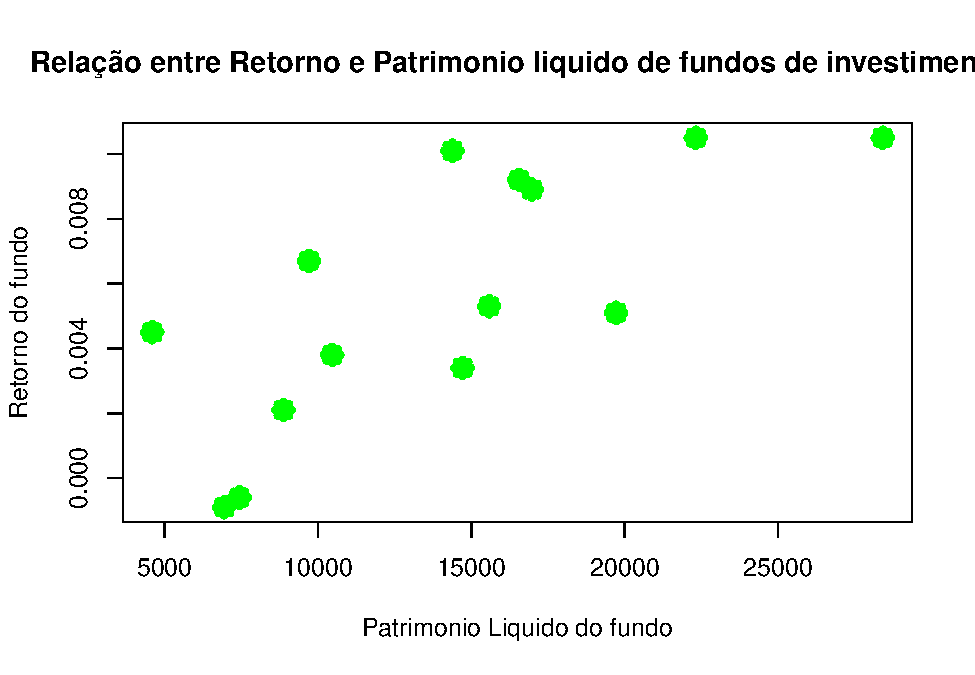
\includegraphics{Aula0R_Exemplo_RMarkdwon_2020_ERE_files/figure-latex/unnamed-chunk-2-1.pdf}

\begin{itemize}
\tightlist
\item
  Questão 2:
\end{itemize}

Crie 6 vetores 2x1 contendo informações sobre média, mediana, mínimo,
máximo, variância o desvio padrão do PL e Ret. E seguida, compile os
vetores em uma única tabela utilizando o comando cbind.data.frame.

\begin{Shaded}
\begin{Highlighting}[]
\NormalTok{media }\OtherTok{\textless{}{-}} \FunctionTok{c}\NormalTok{(}\FunctionTok{mean}\NormalTok{(dados}\SpecialCharTok{$}\StringTok{\textasciigrave{}}\AttributeTok{PL em milhoes}\StringTok{\textasciigrave{}}\NormalTok{),}\FunctionTok{mean}\NormalTok{(dados}\SpecialCharTok{$}\NormalTok{Retorno))}
\NormalTok{mediana }\OtherTok{\textless{}{-}} \FunctionTok{c}\NormalTok{(}\FunctionTok{median}\NormalTok{(dados}\SpecialCharTok{$}\StringTok{\textasciigrave{}}\AttributeTok{PL em milhoes}\StringTok{\textasciigrave{}}\NormalTok{),}\FunctionTok{median}\NormalTok{(dados}\SpecialCharTok{$}\NormalTok{Retorno))}
\NormalTok{minimo }\OtherTok{\textless{}{-}} \FunctionTok{c}\NormalTok{(}\FunctionTok{min}\NormalTok{(dados}\SpecialCharTok{$}\StringTok{\textasciigrave{}}\AttributeTok{PL em milhoes}\StringTok{\textasciigrave{}}\NormalTok{),}\FunctionTok{min}\NormalTok{(dados}\SpecialCharTok{$}\NormalTok{Retorno))}
\NormalTok{maximo }\OtherTok{\textless{}{-}} \FunctionTok{c}\NormalTok{(}\FunctionTok{max}\NormalTok{(dados}\SpecialCharTok{$}\StringTok{\textasciigrave{}}\AttributeTok{PL em milhoes}\StringTok{\textasciigrave{}}\NormalTok{),}\FunctionTok{max}\NormalTok{(dados}\SpecialCharTok{$}\NormalTok{Retorno))}
\NormalTok{desvio\_padrao }\OtherTok{\textless{}{-}} \FunctionTok{c}\NormalTok{(}\FunctionTok{sd}\NormalTok{(dados}\SpecialCharTok{$}\StringTok{\textasciigrave{}}\AttributeTok{PL em milhoes}\StringTok{\textasciigrave{}}\NormalTok{),}\FunctionTok{sd}\NormalTok{(dados}\SpecialCharTok{$}\NormalTok{Retorno))}
\NormalTok{variancia }\OtherTok{\textless{}{-}} \FunctionTok{c}\NormalTok{(}\FunctionTok{var}\NormalTok{(dados}\SpecialCharTok{$}\StringTok{\textasciigrave{}}\AttributeTok{PL em milhoes}\StringTok{\textasciigrave{}}\NormalTok{),}\FunctionTok{var}\NormalTok{(dados}\SpecialCharTok{$}\NormalTok{Retorno))}
\NormalTok{enriched\_data }\OtherTok{\textless{}{-}} \FunctionTok{cbind.data.frame}\NormalTok{(media,mediana,minimo,maximo, desvio\_padrao,variancia)}
\FunctionTok{round\_df}\NormalTok{(enriched\_data,}\DecValTok{5}\NormalTok{)}
\end{Highlighting}
\end{Shaded}

\begin{verbatim}
##         media    mediana    minimo     maximo desvio_padrao      variancia
## 1 14049.57143 14550.5000 4600.0000 28409.0000    6600.05778 43560762.72527
## 2     0.00561     0.0052   -0.0009     0.0105       0.00388        0.00002
\end{verbatim}

\begin{itemize}
\tightlist
\item
  Questão 3:
\end{itemize}

A covariância e correlação entre PL e Ret

\begin{Shaded}
\begin{Highlighting}[]
\NormalTok{covariancia }\OtherTok{\textless{}{-}} \FunctionTok{cov}\NormalTok{(dados}\SpecialCharTok{$}\StringTok{\textasciigrave{}}\AttributeTok{PL em milhoes}\StringTok{\textasciigrave{}}\NormalTok{,dados}\SpecialCharTok{$}\NormalTok{Retorno)}
\NormalTok{correlacao }\OtherTok{\textless{}{-}} \FunctionTok{cor}\NormalTok{(dados}\SpecialCharTok{$}\StringTok{\textasciigrave{}}\AttributeTok{PL em milhoes}\StringTok{\textasciigrave{}}\NormalTok{,dados}\SpecialCharTok{$}\NormalTok{Retorno)}
\end{Highlighting}
\end{Shaded}

\begin{itemize}
\tightlist
\item
  Questão 4:
\end{itemize}

Crie um modelo linear para captar a relação entre Ret e PL. Reti = A +
BPLi + Ei

\begin{Shaded}
\begin{Highlighting}[]
\NormalTok{x }\OtherTok{\textless{}{-}}\NormalTok{ dados}\SpecialCharTok{$}\StringTok{\textasciigrave{}}\AttributeTok{PL em milhoes}\StringTok{\textasciigrave{}}
\NormalTok{y }\OtherTok{\textless{}{-}}\NormalTok{ dados}\SpecialCharTok{$}\NormalTok{Retorno}
\NormalTok{reg }\OtherTok{\textless{}{-}} \FunctionTok{lm}\NormalTok{(y }\SpecialCharTok{\textasciitilde{}}\NormalTok{ x)}
\end{Highlighting}
\end{Shaded}

\begin{itemize}
\tightlist
\item
  Questão 5:
\end{itemize}

Insira no gráfico de dispersão anterior uma linha que representa o
modelo linear na cor azul.

\begin{Shaded}
\begin{Highlighting}[]
\CommentTok{\#Grafico Anterior:}
\FunctionTok{plot}\NormalTok{(dados}\SpecialCharTok{$}\StringTok{\textasciigrave{}}\AttributeTok{PL em milhoes}\StringTok{\textasciigrave{}}\NormalTok{, dados}\SpecialCharTok{$}\NormalTok{Retorno,}
     \AttributeTok{pch  =} \DecValTok{8}\NormalTok{,}
     \AttributeTok{col  =} \StringTok{"green"}\NormalTok{,}
     \AttributeTok{lwd  =} \DecValTok{5}\NormalTok{,}
     \AttributeTok{main =} \StringTok{"Relação entre Retorno e Patrimonio liquido de fundos de investimento"}\NormalTok{,}
     \AttributeTok{xlab =} \StringTok{"Patrimonio Liquido do fundo"}\NormalTok{,}
     \AttributeTok{ylab =} \StringTok{"Retorno do fundo"}\NormalTok{)}
\CommentTok{\#Linha Azul:}
\FunctionTok{abline}\NormalTok{(reg, }\AttributeTok{col=}\DecValTok{4}\NormalTok{)}
\end{Highlighting}
\end{Shaded}

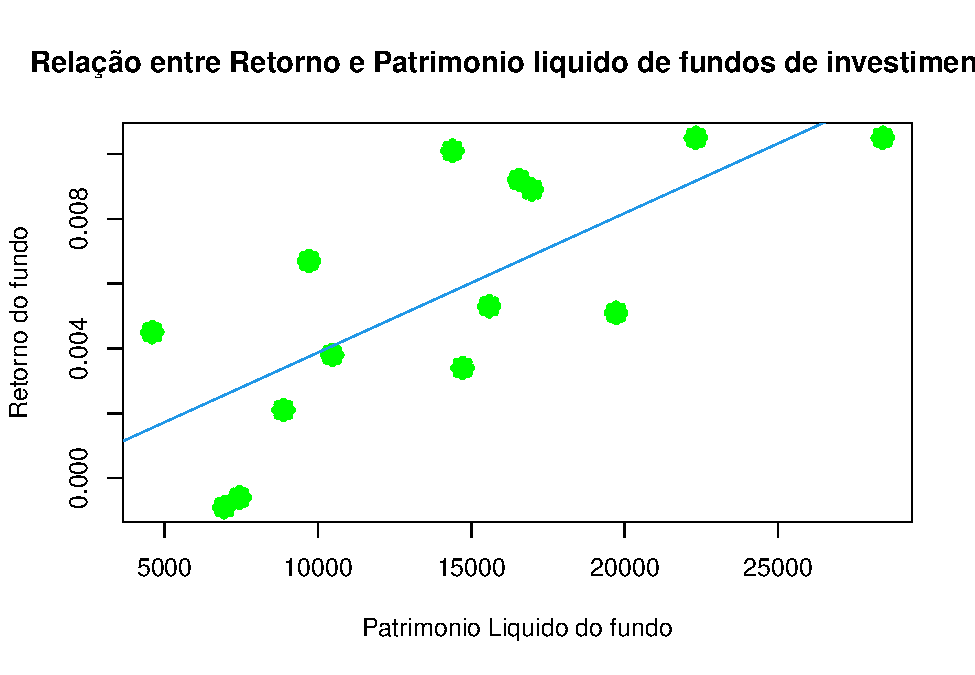
\includegraphics{Aula0R_Exemplo_RMarkdwon_2020_ERE_files/figure-latex/unnamed-chunk-6-1.pdf}

\begin{itemize}
\tightlist
\item
  Questão 6:
\end{itemize}

Mostre o resultado do modelo e a adequabilidade da modelagem.

\begin{verbatim}
## [1] "Coeficiente do intercepto: -0.000429925858032385"
\end{verbatim}

\begin{verbatim}
## [1] "Coeficiente do X: 0.00000043020611717924"
\end{verbatim}

O resultado do modelo são os coeficientes citados a cima.

\begin{itemize}
\tightlist
\item
  Questão 7
\end{itemize}

Analise o poder explicativo do modelo.

\begin{verbatim}
## [1] "R2 do modelo = 0.535012450316333"
\end{verbatim}

O poder explicativo do modelo é 53,5\% o R², ou seja, 53,5\% dos
resultados dos fundos podem ser explicados pelo fator PL

\begin{itemize}
\tightlist
\item
  Questão 8
\end{itemize}

Analise o significado do valor e significância de 𝛼 e 𝛽 gerados a um
nível de significância de 5\%

\begin{Shaded}
\begin{Highlighting}[]
\FunctionTok{paste}\NormalTok{(}\StringTok{"P valor do intercepto="}\NormalTok{,reg\_slm}\SpecialCharTok{$}\NormalTok{coefficients[}\DecValTok{1}\NormalTok{,}\DecValTok{4}\NormalTok{])}
\end{Highlighting}
\end{Shaded}

\begin{verbatim}
## [1] "P valor do intercepto= 0.813787589294106"
\end{verbatim}

\begin{Shaded}
\begin{Highlighting}[]
\FunctionTok{paste}\NormalTok{(}\StringTok{"P valor do Coeficiente="}\NormalTok{,reg\_slm}\SpecialCharTok{$}\NormalTok{coefficients[}\DecValTok{2}\NormalTok{,}\DecValTok{4}\NormalTok{])}
\end{Highlighting}
\end{Shaded}

\begin{verbatim}
## [1] "P valor do Coeficiente= 0.00294942039128462"
\end{verbatim}

O p valor do intercepto é maior que 5\% por isso faz a variavel ser
pouco efetiva ao modelo tendo alta chance de fazer parte de uma hipotese
nula,já o p valor do coeficiente é menor que 5\%, por isso é
significante

\begin{itemize}
\tightlist
\item
  Questão 9
\end{itemize}

Crie uma expectativa de Ret para um fundo com PL igual a R\$7.800,00.

\begin{Shaded}
\begin{Highlighting}[]
\NormalTok{result }\OtherTok{\textless{}{-}}\NormalTok{ reg\_slm}\SpecialCharTok{$}\NormalTok{coefficients[}\DecValTok{1}\NormalTok{,}\DecValTok{1}\NormalTok{] }\SpecialCharTok{+}\NormalTok{ reg\_slm}\SpecialCharTok{$}\NormalTok{coefficients[}\DecValTok{2}\NormalTok{,}\DecValTok{1}\NormalTok{] }\SpecialCharTok{*} \DecValTok{7800}
\FunctionTok{paste}\NormalTok{(}\StringTok{"Retorno esperado= "}\NormalTok{,}\FunctionTok{round}\NormalTok{(result }\SpecialCharTok{*} \DecValTok{100}\NormalTok{,}\DecValTok{3}\NormalTok{),}\StringTok{"\%"}\NormalTok{,}\AttributeTok{sep=}\StringTok{""}\NormalTok{)}
\end{Highlighting}
\end{Shaded}

\begin{verbatim}
## [1] "Retorno esperado= 0.293%"
\end{verbatim}

\begin{itemize}
\tightlist
\item
  Questão 10
\end{itemize}

Faça uma nova estimação considerando agora um modelo sem intercepto (𝛼 =
0).

\begin{Shaded}
\begin{Highlighting}[]
\NormalTok{x }\OtherTok{\textless{}{-}}\NormalTok{ dados}\SpecialCharTok{$}\StringTok{\textasciigrave{}}\AttributeTok{PL em milhoes}\StringTok{\textasciigrave{}}
\NormalTok{y }\OtherTok{\textless{}{-}}\NormalTok{ dados}\SpecialCharTok{$}\NormalTok{Retorno}
\NormalTok{regSemAlfa }\OtherTok{\textless{}{-}} \FunctionTok{lm}\NormalTok{(y }\SpecialCharTok{\textasciitilde{}}\NormalTok{ x }\SpecialCharTok{{-}} \DecValTok{1}\NormalTok{)}
\end{Highlighting}
\end{Shaded}

\begin{itemize}
\tightlist
\item
  Questão 11
\end{itemize}

Insira no gráfico de dispersão a reta deste novo modelo na cor vermelha.

\begin{Shaded}
\begin{Highlighting}[]
\CommentTok{\#Grafico Anterior:}
\FunctionTok{plot}\NormalTok{(dados}\SpecialCharTok{$}\StringTok{\textasciigrave{}}\AttributeTok{PL em milhoes}\StringTok{\textasciigrave{}}\NormalTok{, dados}\SpecialCharTok{$}\NormalTok{Retorno,}
     \AttributeTok{pch  =} \DecValTok{8}\NormalTok{,}
     \AttributeTok{col  =} \StringTok{"green"}\NormalTok{,}
     \AttributeTok{lwd  =} \DecValTok{5}\NormalTok{,}
     \AttributeTok{main =} \StringTok{"Relação entre Retorno e Patrimonio liquido de fundos de investimento"}\NormalTok{,}
     \AttributeTok{xlab =} \StringTok{"Patrimonio Liquido do fundo"}\NormalTok{,}
     \AttributeTok{ylab =} \StringTok{"Retorno do fundo"}\NormalTok{)}
\CommentTok{\#Linha Azul:}
\FunctionTok{abline}\NormalTok{(reg, }\AttributeTok{col=}\DecValTok{4}\NormalTok{)}

\CommentTok{\#Linha vermelha nova:}
\FunctionTok{abline}\NormalTok{(regSemAlfa, }\AttributeTok{col=}\StringTok{"red"}\NormalTok{)}
\end{Highlighting}
\end{Shaded}

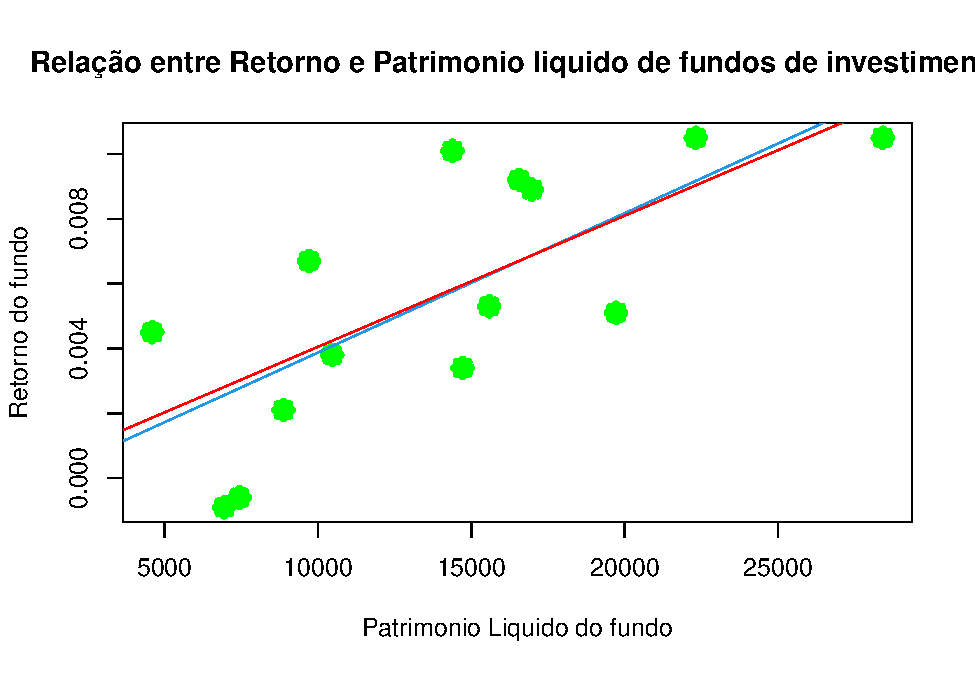
\includegraphics{Aula0R_Exemplo_RMarkdwon_2020_ERE_files/figure-latex/unnamed-chunk-12-1.pdf}

\begin{itemize}
\tightlist
\item
  Questão 12
\end{itemize}

Analise a validade do modelo, poder explicativo do modelo e a magnitude
e significância do B

\begin{Shaded}
\begin{Highlighting}[]
\NormalTok{regSemAlfa\_slm }\OtherTok{\textless{}{-}} \FunctionTok{summary}\NormalTok{(regSemAlfa)}
\FunctionTok{paste}\NormalTok{(}\StringTok{"R2 do novo modelo="}\NormalTok{,regSemAlfa\_slm}\SpecialCharTok{$}\NormalTok{r.squared)}
\end{Highlighting}
\end{Shaded}

\begin{verbatim}
## [1] "R2 do novo modelo= 0.856351702042533"
\end{verbatim}

\begin{Shaded}
\begin{Highlighting}[]
\FunctionTok{paste}\NormalTok{(}\StringTok{"P valor do novo modelo="}\NormalTok{,}\FunctionTok{glance}\NormalTok{(regSemAlfa)}\SpecialCharTok{$}\NormalTok{p.value)}
\end{Highlighting}
\end{Shaded}

\begin{verbatim}
## [1] "P valor do novo modelo= NA"
\end{verbatim}

\begin{Shaded}
\begin{Highlighting}[]
\FunctionTok{paste}\NormalTok{(}\StringTok{"P valor do novo X="}\NormalTok{,regSemAlfa\_slm}\SpecialCharTok{$}\NormalTok{coefficients[,}\DecValTok{4}\NormalTok{])}
\end{Highlighting}
\end{Shaded}

\begin{verbatim}
## [1] "P valor do novo X= 0.00000077269311622811"
\end{verbatim}

\begin{Shaded}
\begin{Highlighting}[]
\CommentTok{\#Printar R2, e o p valor de x}
\end{Highlighting}
\end{Shaded}

O poder explicativo (R2) foi para 85\% sendo um modelo mais adequado que
o primeiro. O P Valor de x dele se tornou estatisticamente igual a 0 e o
P Valor do modelo se tornou estatisticamente igual 0

\begin{itemize}
\tightlist
\item
  Questão 13
\end{itemize}

Compare os resultados dos dois modelos e justifique em termos
estatísticos qual dos dois modelos é mais adequado.

\begin{Shaded}
\begin{Highlighting}[]
\FunctionTok{paste}\NormalTok{(}\StringTok{"R2 do novo modelo="}\NormalTok{,regSemAlfa\_slm}\SpecialCharTok{$}\NormalTok{r.squared)}
\end{Highlighting}
\end{Shaded}

\begin{verbatim}
## [1] "R2 do novo modelo= 0.856351702042533"
\end{verbatim}

\begin{Shaded}
\begin{Highlighting}[]
\FunctionTok{paste}\NormalTok{(}\StringTok{"P valor do novo modelo="}\NormalTok{,}\FunctionTok{glance}\NormalTok{(regSemAlfa)}\SpecialCharTok{$}\NormalTok{p.value)}
\end{Highlighting}
\end{Shaded}

\begin{verbatim}
## [1] "P valor do novo modelo= NA"
\end{verbatim}

\begin{Shaded}
\begin{Highlighting}[]
\FunctionTok{paste}\NormalTok{(}\StringTok{"R2 do antigo modelo="}\NormalTok{,reg\_slm}\SpecialCharTok{$}\NormalTok{r.squared)}
\end{Highlighting}
\end{Shaded}

\begin{verbatim}
## [1] "R2 do antigo modelo= 0.535012450316333"
\end{verbatim}

\begin{Shaded}
\begin{Highlighting}[]
\FunctionTok{paste}\NormalTok{(}\StringTok{"P valor do Antigo modelo="}\NormalTok{,}\FunctionTok{glance}\NormalTok{(reg)}\SpecialCharTok{$}\NormalTok{p.value)}
\end{Highlighting}
\end{Shaded}

\begin{verbatim}
## [1] "P valor do Antigo modelo= 0.00294942039128463"
\end{verbatim}

\begin{Shaded}
\begin{Highlighting}[]
\FunctionTok{paste}\NormalTok{(}\StringTok{"Melhoria do R2 = "}\NormalTok{, (regSemAlfa\_slm}\SpecialCharTok{$}\NormalTok{r.squared }\SpecialCharTok{{-}}\NormalTok{ reg\_slm}\SpecialCharTok{$}\NormalTok{r.squared)}\SpecialCharTok{/}\NormalTok{ reg\_slm}\SpecialCharTok{$}\NormalTok{r.squared }\SpecialCharTok{*}\DecValTok{100}\NormalTok{, }\StringTok{"\%"}\NormalTok{, }\AttributeTok{sep=}\StringTok{""}\NormalTok{)}
\end{Highlighting}
\end{Shaded}

\begin{verbatim}
## [1] "Melhoria do R2 = 60.0620137972871%"
\end{verbatim}

\begin{itemize}
\tightlist
\item
  Questão 14
\end{itemize}

Responda a seu cliente qual a melhor opção de fundo para investir, os
menores ou os maiores

Mesmo com a regressão mais fraca, já demonstrava uma tendencia de fundos
com patrimonios maiores terem mais retorno. Com a regressão mais forte a
tendencia foi confirmada, segundo o coeficiente de X
\texttt{\{r\}regSemAlfa\_slm\$coefficients{[}1{]}}, a cada variação de 1
milhão de PL do fundo, o rendimento tende a ser
\texttt{\{r\}regSemAlfa\_slm\$coefficients{[}1{]}} maior, alem do mais a
relação é positiva, ou seja, nesse caso, maior melhor.

\begin{itemize}
\tightlist
\item
  Questão 15:
\end{itemize}

Por fim, levante hipóteses sobre outros fatores que podem impactar o ret
de fundos de investimentos.

Levando em consideração o artigo: {[}link{]}
(\url{https://convibra.org/congresso/res/uploads/pdf/artigo23093_20201802.pdf})
O \emph{Patrimonio Liquido logaritimizado} apresenta uma \emph{relação
negativa}, juntamente com a \emph{Taxa de administração} e a \emph{Idade
do fundo}, já por outro lado, apresentam uma \emph{relação positiva} as
variaveis \emph{Taxa de performance} a \emph{Taxa de administração ao
quadrado}

\end{document}
